% Modern editorial, markup and figure/layout contributions: CC-BY-SA-4.0.
% Historical text and illustrations: Leonhard Euler (1744), public domain.
% Component scope and upstream attribution: see RIGHTS.md.
% Manual vector redraw from E65 Tabula II, Fig. 20.
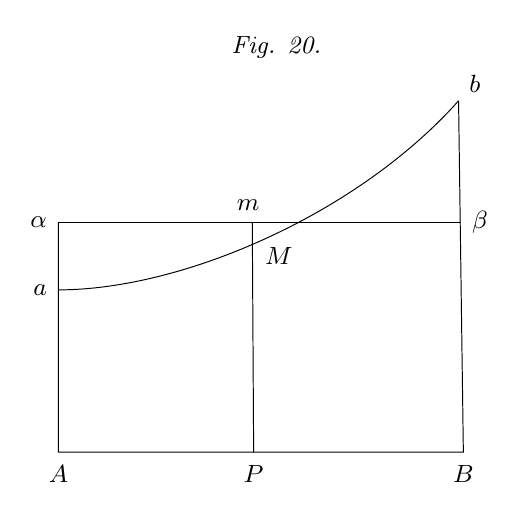
\begin{tikzpicture}[x=1cm,y=1cm,line width=.35pt,font=\small]
\draw (0.3318,2.9341)--(0.3318,0.0175)--(5.4752,0.0175)--(5.4141,4.4797);
\draw (0.3318,2.9341)--(5.4403,2.9341);
\draw (2.8118,0.0175)--(2.7944,2.9341);
\draw (0.3318,2.0783) .. controls (1.9211,2.0783) and (4.1392,3.0476) .. (5.4141,4.4797);
\node[anchor=north,inner sep=1pt] at (0.3318,-0.1135) {$A$};
\node[anchor=north,inner sep=1pt] at (5.4752,-0.1135) {$B$};
\node[anchor=north,inner sep=1pt] at (2.8118,-0.1135) {$P$};
\node[anchor=east,inner sep=1pt] at (0.2270,2.0783) {$a$};
\node[anchor=south west,inner sep=1pt] at (5.5101,4.5408) {$b$};
\node[anchor=east,inner sep=1pt] at (0.2270,2.9341) {$\alpha$};
\node[anchor=west,inner sep=1pt] at (5.5451,2.9341) {$\beta$};
\node[anchor=south,inner sep=1pt] at (2.7420,3.0476) {$m$};
\node[anchor=north west,inner sep=1pt] at (2.9166,2.6634) {$M$};
\node[anchor=south] at (3.1000,4.8901) {\textit{Fig. 20.}};
\end{tikzpicture}
